\documentclass[parskip]{scrartcl}
\usepackage{tikz}
\usetikzlibrary{3d, calc, shapes.geometric, positioning, shadows.blur, decorations.pathreplacing, shapes.multipart, shapes.symbols, fit, backgrounds}
\usepackage{pgfplots}
\usepackage[margin=40mm]{geometry}
\pgfplotsset{compat=1.18}
\usepackage{xcolor}
\usepackage{tikz-3dplot}
\usepackage{draculatheme}


% Define colors for different components
% \definecolor{softmax}{RGB}{204, 231, 207}       % Light Green
% \definecolor{linear}{RGB}{219, 223, 239}        % Periwinkle
% \definecolor{addnorm}{RGB}{242, 244, 193}       % Light Yellow
% \definecolor{feedforward}{RGB}{193, 232, 247}   % Light Turquoise
% \definecolor{multi-head}{RGB}{255, 226, 187}    % Light Orange
% \definecolor{embedding}{RGB}{252, 224, 225}     % Rose
% \definecolor{Nx}{RGB}{243, 243, 244}            % Very Light Gray

% Darker color definitions
\definecolor{softmax}{RGB}{124,151,127}     % from (204,231,207)
\definecolor{linear}{RGB}{139,143,159}      % from (219,223,239)
\definecolor{addnorm}{RGB}{162,164,113}     % from (242,244,193)
\definecolor{feedforward}{RGB}{113,152,167} % from (193,232,247)
\definecolor{multi-head}{RGB}{175,146,107}  % from (255,226,187)
\definecolor{embedding}{RGB}{172,144,145}   % from (252,224,225)
\definecolor{Nx}{RGB}{163,163,164}          % from (243,243,244)

\def \benddistance {1cm} % For bends inside the Nx blocks

\begin{document}

\begin{center}
    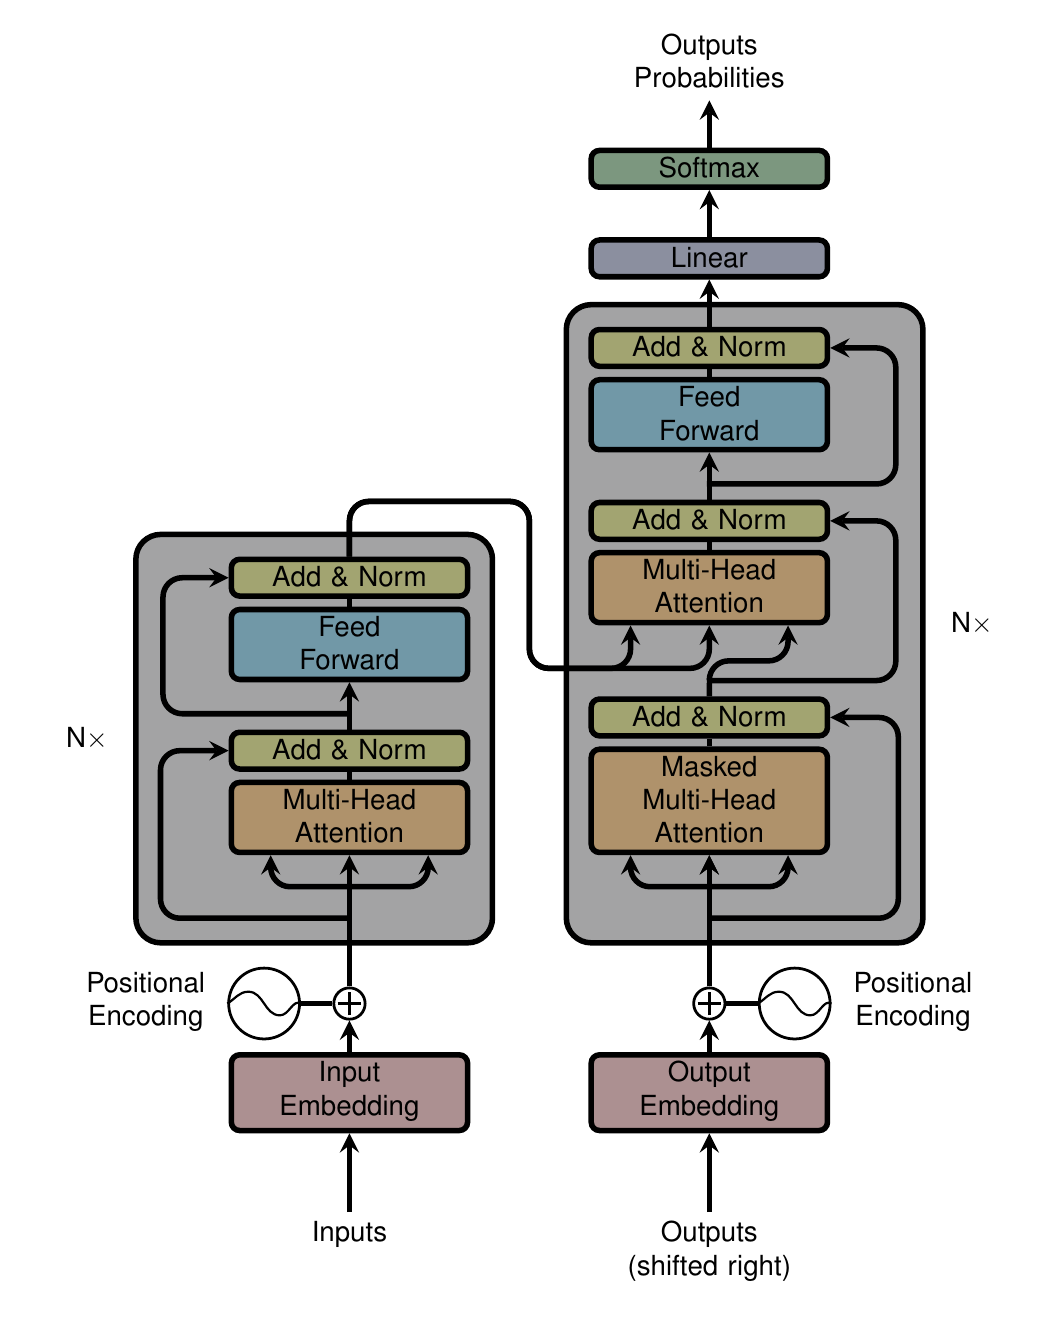
\begin{tikzpicture}[
        thick,
        processing/.style={draw, minimum width=3cm,  align=center, anchor=north, rounded corners=3pt, text width=2.6cm, font=\fontfamily{phv}\selectfont, text height=1.5ex, line width=2pt},
        pointers/.style={thick, -stealth, line width=2pt},
        fit_rectangle/.style={draw, minimum width=3cm,  align=center, anchor=north, rounded corners=9pt, font=\fontfamily{phv}\selectfont, inner sep = 8pt, line width=2pt, fill=Nx},
    ]
    
    % --------- NODES ----------   
        % Left Side
            \node[processing,draw = none] (inputs) {Inputs\\\phantom{(shifted right)}};
            \node[processing, above=1cm of inputs, fill=embedding] (input_embed) {Input\\ Embedding};
            \node[processing, above=2.5cm of input_embed, fill=multi-head] (multihead) {Multi-Head\\ Attention};
            \node[processing, above=0.1cm of multihead, fill=addnorm] (addnorm1) {Add \& Norm};
            \node[processing, above=0.6cm of addnorm1, fill=feedforward] (feedforward1) {Feed \\Forward};
            \node[processing, above=0.1cm of feedforward1, fill=addnorm] (addnorm3) {Add \& Norm};

        % Right Side
            \node[processing, right=1.5cm of inputs, draw=none] (outputs) {Outputs\\(shifted right)};
            \node[processing, above=1cm of outputs, fill=embedding] (output_embed) {Output\\ Embedding};
            \node[processing, above=2.5cm of output_embed, fill=multi-head] (multihead2) {Masked \\Multi-Head\\ Attention};
            \node[processing, above=0.1cm of multihead2, fill=addnorm] (addnorm2) {Add \& Norm};
            \node[processing, above=0.9cm of addnorm2, fill=multi-head] (multihead3) {Multi-Head\\ Attention};
            \node[processing, above=0.1cm of multihead3, fill=addnorm] (addnorm4) {Add \& Norm};
            \node[processing, above=0.6cm of addnorm4, fill=feedforward] (feedforward2) {Feed \\Forward};
            \node[processing, above=0.1cm of feedforward2, fill=addnorm] (addnorm5) {Add \& Norm};
            \node[processing, above=0.6cm of addnorm5, fill=linear] (linear) {Linear};
            \node[processing, above=0.6cm of linear, fill=softmax] (softmax) {Softmax};
            \node[processing, draw=none, above=0.6cm of softmax] (outputs2) {Outputs\\Probabilities};

    % -------- PLUSES ----------

        % Draw plus for input_embed
        \coordinate (plus1) at ($(input_embed.north)+(0,0.4cm)$);

        \node[circle, draw, inner sep = 4pt, above=.4cm of input_embed,line width = 1pt] (plus1) {};
        \draw[line width=1pt] ($(plus1)+(-0.15cm,0)$) -- ($(plus1)+(0.15cm,0)$);
        \draw[line width=1pt] ($(plus1)+(0,-0.15cm)$) -- ($(plus1)+(0,0.15cm)$);

        % Draw plus for output_embed
        \coordinate (plus2) at ($(output_embed.north)+(0,0.4cm)$);
        \node[circle, draw, inner sep = 4pt, above=.4cm of output_embed,line width = 1pt] (plus2) {};
        \draw[line width=1pt] ($(plus2)+(-0.15cm,0)$) -- ($(plus2)+(0.15cm,0)$);
        \draw[line width=1pt] ($(plus2)+(0,-0.15cm)$) -- ($(plus2)+(0,0.15cm)$);

        % Positional Encoding Circle
        \node[circle, draw, minimum size=0.9cm, 
        left=0.4cm of plus1, line width=1pt] (pos_enc1) {};

        \node[circle, draw, minimum size=0.9cm, 
        right=0.4cm of plus2, line width=1pt] (pos_enc2) {};

        % Positional Encoding Text
        \node[processing, draw = none, left=-0.5cm of pos_enc1] (pos_enc1_text) {Positional\\Encoding};    
        
        \node[processing, draw = none, right=-0.5cm of pos_enc2] (pos_enc2_text) {Positional\\Encoding}; 

        % Connect positional encoding to addition
        \draw[line width = 2pt] (pos_enc1) -- (plus1);
        \draw[line width = 2pt] (pos_enc2) -- (plus2);

        % Draw the wavy lines in the positional encoding circles
        \draw (pos_enc1.west) to[out=30, in=180] ($(pos_enc1.center) + (-0.2,0.15)$)
        to[out=0, in=180] ($(pos_enc1.center) + (0.2,-0.15)$)
        to[out=0, in=150] (pos_enc1.east);
        
        \draw (pos_enc2.west) to[out=30, in=180] ($(pos_enc2.center) + (-0.2,0.15)$)
        to[out=0, in=180] ($(pos_enc2.center) + (0.2,-0.15)$)
        to[out=0, in=150] (pos_enc2.east);
    
    % --------- ARROWS ---------- 

        % Arrows outside the Nx blocks
            % Left side
                \draw[pointers] (inputs.north) -- (input_embed.south);
                \draw[pointers] (input_embed.north) -- (plus1.south);
                % \draw[line width = 2pt] (plus1.north) -- (multihead.south);

            % Right side (bottom)
                \draw[pointers] (outputs.north) -- (output_embed.south);
                \draw[pointers] (output_embed.north) -- (plus2.south);
                \draw[pointers] (plus2.north) -- (multihead2.south);

            % Right side (top)
                \draw[pointers] (linear.north) -- (softmax.south);
                \draw[pointers] (softmax.north) -- (outputs2.south);

        % Lines conecting nodes inside the Nx rectangles
            % Left side
                \draw[line width = 2pt] (multihead.north) -- (addnorm1.south);
                \draw[pointers] (addnorm1.north) -- (feedforward1.south);
                \draw[line width = 2pt] (feedforward1.north) -- (addnorm3.south);

            % Right side
                \draw[line width = 2pt] (multihead2.north) -- (addnorm2.south);
                % \draw[pointers] (addnorm2.north) -- (multihead3.south);
                \draw[line width = 2pt] (multihead3.north) -- (addnorm4.south);
                \draw[pointers] (addnorm4.north) -- (feedforward2.south);
                \draw[line width = 2pt] (feedforward2.north) -- (addnorm5.south);
                \draw[pointers] (addnorm5.north) -- (linear.south);

        % Curved Arrows

        % Left side
            % Dummy nodes for forking and bending
                \node[draw, inner sep = 0pt, fill = black] (left_encoder_fork_bottom) at ($(multihead.south)+(0,-.4cm)$) {};
                \node[draw, inner sep = 0pt, fill = black] (left_encoder_fork_bottom_lower) at ($(left_encoder_fork_bottom)+(0,-.4cm)$) {};
                \node[draw=none, inner sep = 0pt] (encoder_bend) at ($(left_encoder_fork_bottom_lower) +(-2.4cm, 0)$) {};
                \node[draw, inner sep = 0pt, fill = black] (left_feed_forward_bottom) at ($(feedforward1.south)+(0,-.4cm)$) {}; 

            % Fork into multiple arrows up to the addnorm1 node's left (bottom)
                % Draw a single arrow from plus1 to the dummy node
                \draw[line width = 2pt] (plus1.north) -- (left_encoder_fork_bottom);
                
                % Fork into multiple arrows up to the multihead node's bottom
                \coordinate (llthird) at ($(multihead.south)+(-\benddistance,0)$);
                \coordinate (lrthird) at ($(multihead.south)+(\benddistance,0)$);

                \draw[pointers, rounded corners = 7pt] (left_encoder_fork_bottom.east) -| (lrthird);
                \draw[pointers, rounded corners=5pt] (plus1.north) -- (multihead.south);
                \draw[pointers, rounded corners=7pt] (left_encoder_fork_bottom.west) -| (llthird);

                \draw[pointers, rounded corners=7pt]
                (left_encoder_fork_bottom_lower)
                -- ++(-2.4cm, 0)  % move left by 2.4cm
                |- (addnorm1.west);

            % Bend into the addnorm1 node's left side (top)
                \draw[pointers, rounded corners=7pt] 
                (left_feed_forward_bottom.east) 
                -- ++(-2.4cm, 0) % move left by 2.4cm
                |- (addnorm3.west);


        % Right side
            % Dummy nodes for forking and bending
            \node[draw, inner sep = 0pt, fill = black] (decoder_fork_bottom) at ($(multihead2.south)+(0,-.4cm)$) {};
            \node[draw, inner sep = 0pt, fill = black] (right_encoder_fork_bottom) at ($(decoder_fork_bottom)+(0,-.4cm)$) {};
            \node[draw, inner sep = 0pt] (decoder_bend) at ($(right_encoder_fork_bottom) +(2.4cm, 2)$) {};
            \node[draw, inner sep = 0pt, fill = black] (right_feed_forward_bottom1) at ($(addnorm2.north)+(0,.2cm)$) {};
            \node[draw, inner sep = 0pt, fill = black] (right_feed_forward_bottom2) at ($(feedforward2.south)+(0,-.4cm)$) {}; 

            % Fork into multiple arrows up to the addnorm2 node's right (bottom)
                % Draw a single arrow from plus2 to the dummy node
                \draw[line width = 2pt] (plus2.north) -- (decoder_fork_bottom);
                
                % Fork into multiple arrows up to the multihead2 node's bottom
                \coordinate (rlthird1) at ($(multihead2.south)+(-\benddistance,0)$);
                \coordinate (rrthird1) at ($(multihead2.south)+(\benddistance,0)$);

                \draw[pointers, rounded corners = 7pt] (decoder_fork_bottom.east) -| (rrthird1);
                \draw[pointers, rounded corners=5pt] (plus2.north) -- (multihead2.south);
                \draw[pointers, rounded corners=7pt] (decoder_fork_bottom.west) -| (rlthird1);

                \coordinate(rlthird2) at ($(multihead3.south)+(-\benddistance,0)$);
                \coordinate(rrthird2) at ($(multihead3.south)+(\benddistance,0)$);

                % \draw[pointers, rounded corners = 7pt] (right_feed_forward_bottom1.north) -| (rrthird2);

                \draw[pointers, rounded corners=7pt]
                (right_encoder_fork_bottom)
                -- ++(2.4cm, 0)  % move right by 2.4cm
                |- (addnorm2.east);

                \draw[pointers, rounded corners=7pt]
                (right_feed_forward_bottom1.west)
                -- ++(2.4cm, 0)
                |- (addnorm4.east);

                \draw[pointers, rounded corners=7pt]
                (right_feed_forward_bottom2.west)
                -- ++(2.4cm, 0)
                |- (addnorm5.east);

                \draw[pointers, rounded corners=7pt]
                (addnorm2) -- (right_feed_forward_bottom1)
                -- ++(0,.25cm) coordinate (midA)
                -| (rrthird2);

        % Nx Blocks
        \begin{pgfonlayer}{background}
            \node[fit_rectangle, fit=(multihead) (addnorm1) (feedforward1) (addnorm3) (left_encoder_fork_bottom_lower) (encoder_bend)] (encoder_block) {};

            \node[fit_rectangle, fit=(multihead2) (addnorm2) (multihead3) (addnorm4) (feedforward2) (addnorm5) (right_encoder_fork_bottom) (decoder_bend)] (decoder_block) {};
        \end{pgfonlayer}
        % Add Nx labels
        \node[anchor= west, font=\fontfamily{phv}\selectfont, left=0.2cm of encoder_block.west] {N$\times$};
        \node[anchor = east, font=\fontfamily{phv}\selectfont, right=0.2cm of decoder_block.east] (Nx) {N$\times$};

        
        \coordinate (exit_left_box)    at ($(addnorm3.north)+(0,0.7cm)$); % go up out of left Nx box
        \coordinate (between_boxes)    at ($(exit_left_box)+(2.285cm,0)$); % travel left-to-right in between
        \coordinate (enter_right_box)  at ($(between_boxes)+(0,-2.12cm)$); % move down near the right Nx box

        \draw[pointers, rounded corners=7pt]
            (addnorm3.north)
            -- (exit_left_box)
            -- (between_boxes)
            -- (enter_right_box)
            -| (rlthird2);

        \draw[pointers, rounded corners=7pt]
        (addnorm3.north)
        -- (exit_left_box)
        -- (between_boxes)
        -- (enter_right_box)
        -| (multihead3.south);

    
    \end{tikzpicture}
    \end{center}
\end{document}